In the following diagram, the mentioned components are more closely examined, with the main focus on the application server. While describing the parts, the notation will be the interface they are providing in order to be more general, because there may be one or more different implementations of the same service within the server. The components shown here communicate with each other and work together to complete certain user requests.
\begin{figure}[H]
	\begin{center}
		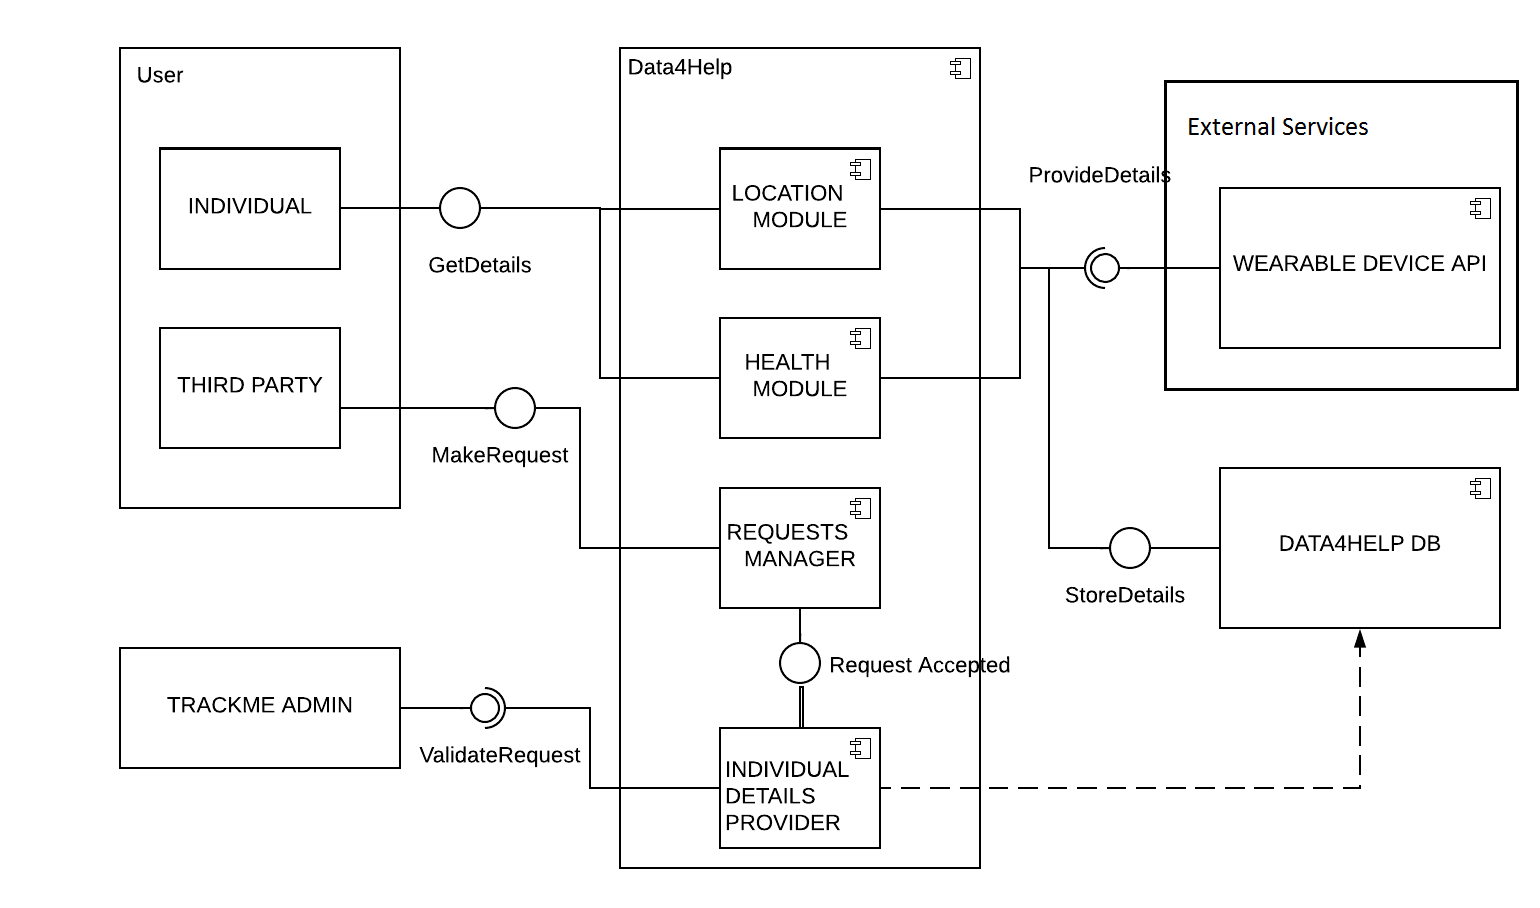
\includegraphics[width=\textwidth]{./DD_Diagrams/ComponentData4Help.png}
      	\caption{Component Diagram for Data4Help Service}
        \label{TrackMe_c1}
	\end{center}
\end{figure}
The location and health is taken from the user by the \textit{GetDetails Interface} with the help of the api of the wearable device by \textit{ProvideDetails Interface}, which the individual selects from the list of compatible devices during registration. The details of the individual is then stored in the Data4Help database using \textit{StoreDetails Interface}.\newline
The thirdparty makes the request to access individual's data which is done by \textit{MakeRequest Interface}.\newline
The TrackMe Admin then validates the third party request and sends it to user to accept/reject or accepts/rejects himself according to the type of requests by \textit{ValidateRequest Interface}.\newline
If the request is accepted the user gets the access of the individual's details which uses the Data4Help Database in order to extract individual's details.
\begin{figure}[H]
	\begin{center}
		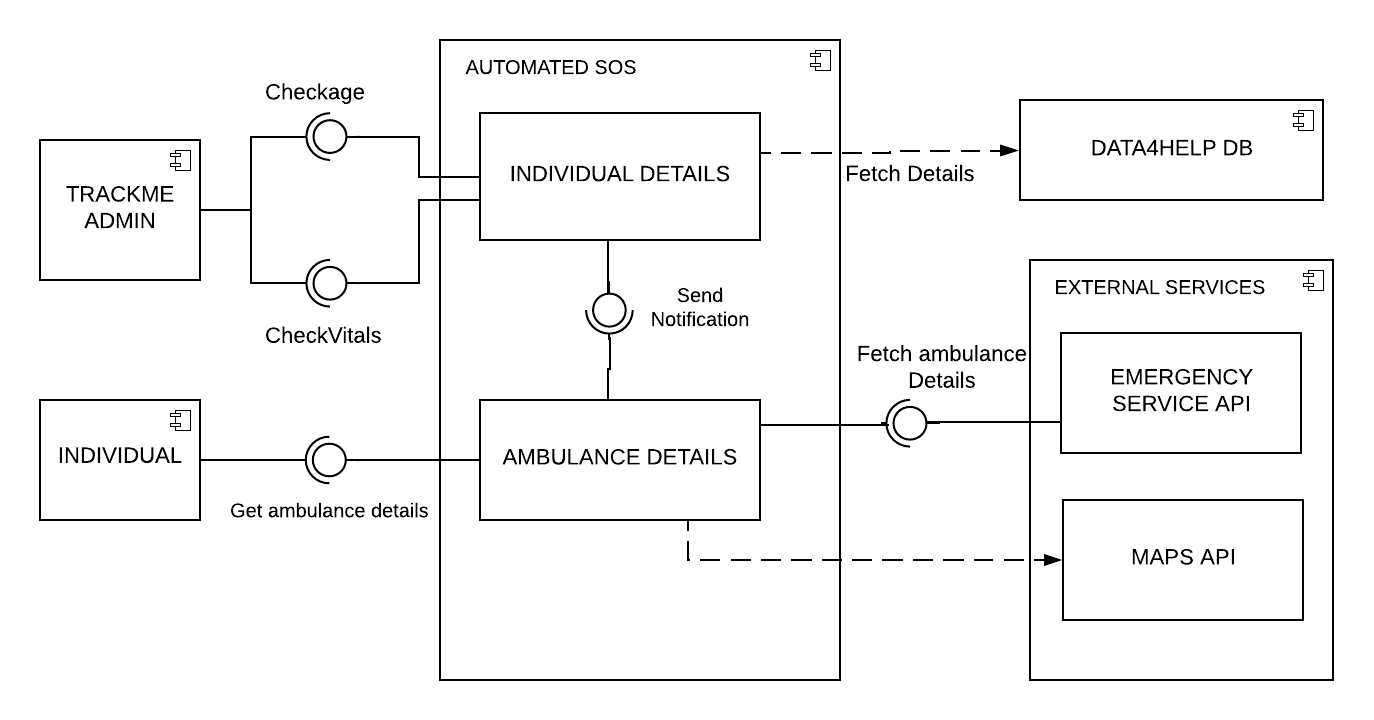
\includegraphics[width=\textwidth]{./DD_Diagrams/ComponentAutomatedSOS.png}
      	\caption{Component Diagram for AutomatedSOS Service}
        \label{TrackMe_c2}
	\end{center}
\end{figure}
Trackme checks the age of the user in order to know whether they are eligible for this service using \textit{CheckAge Interface}. TrackMe checks the vitals to know about the emergency condition using \textit{CheckVitals Interface} which is fetched from the Data4Help Database.\newline 
If the emergency situation is acknowledged the admin sends notification using \textit{SendNotification Interface} .\newline
The Individual receives the Ambulance Details by \textit{GetAmbulanceDetails Interface} and can track the ambulance whose information is fetched from the emergency Service API using \textit{FetchAmbulanceDetails Interface} and uses Maps API to show the map.
\begin{figure}[H]
	\begin{center}
		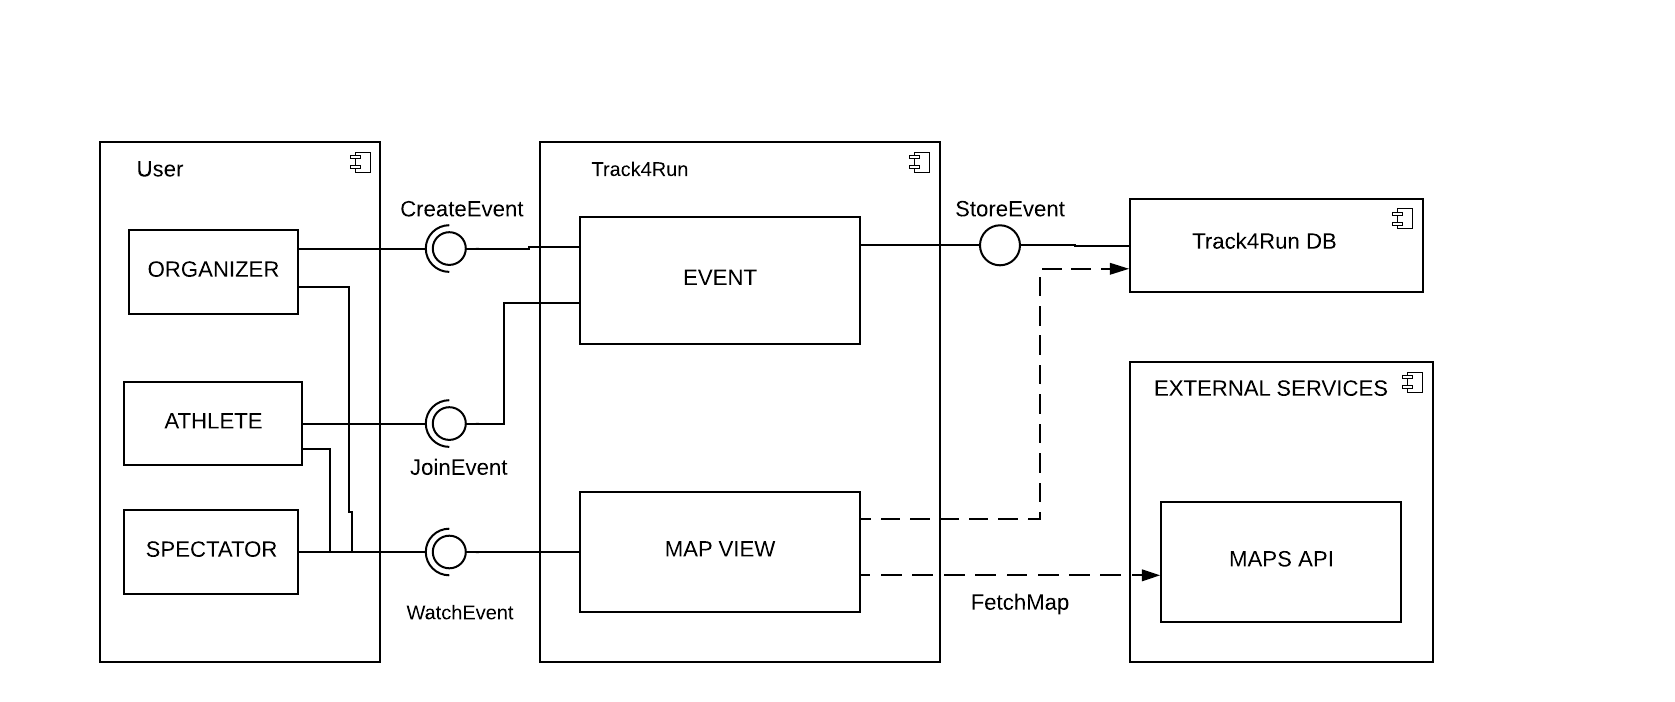
\includegraphics[width=\textwidth]{./DD_Diagrams/ComponentTrack4Run.png}
      	\caption{Component Diagram for Track4Run Service}
        \label{TrackMe_c3}
	\end{center}
\end{figure}
The organizer creates an event which the athlete joins using \textit{CreateEvent Interface} and \textit{JoinEvent Interface} respectively. The details of the event is store din the Track4Run Daatabase using \textit{StoreEvent Interface} which is used by Map view to show the details on map. The organizer, athlete and Spectator can watch the race in a map using \textit{WatchEvent Interface} which uses Map API to fetch the map.
\begin{figure}[H]
	\begin{center}
		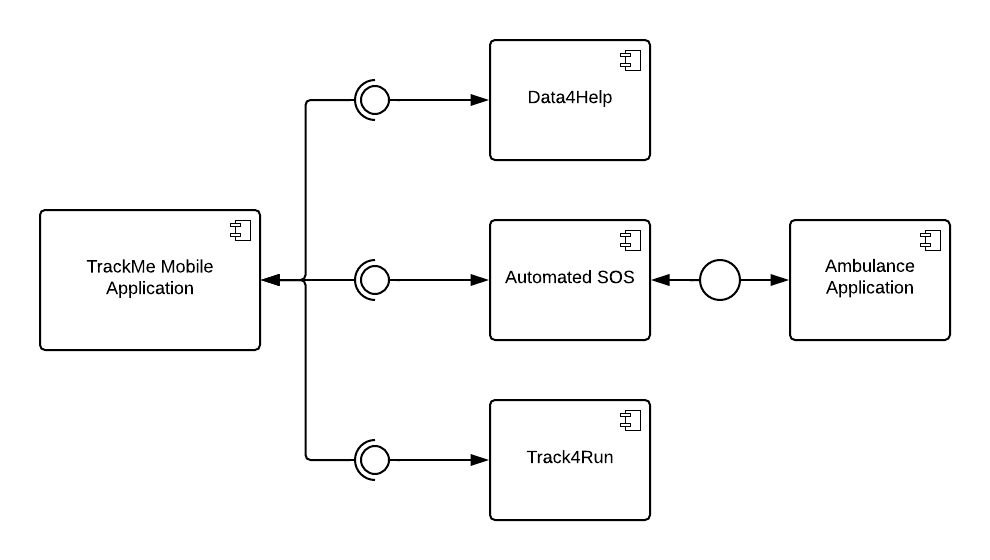
\includegraphics[width=\textwidth]{./DD_Diagrams/Component.png}
      \caption{Main Component Diagram}
        \label{TrackMe_c0}
	\end{center}
\end{figure}
The main component is divided into three subcomponents which are shown separately to avoid unreadability. All the three subcomponents are the services which is being provided by the TrackMe Application.\newline
The Ambulance Application is a separate application developed explicitly for the ambulance drivers where they receive individuals details through push notification. It is connected to Automated SOS service for exchange of information of ambulance and individual respectively.